\chapter{哈密顿方程}
\label{ch:4}

\section*{4.1  勒让德变换}

函数 $f$（$u_s$ 的函数）到 $g$（$v_s$ 的函数）的勒让德变换（Legendre transformation）可通过如下方式定义 $g$ 来实现：
$$
g = \sum_{i=1}^{n} u_i v_i - f.
\eqno\hbox{(4.2)}
$$
乍一看，你也许会认为 $g$ 既是 $u_s$ 又是 $v_s$ 的函数，但取它的定义式的微分，你就会明白 $g$ 只是 $v_s$ 的函数。即
$$
\begin{aligned}
dg &= \sum_{i=1}^{n} (u_i\,dv_i + v_i\,du_i) - \sum_{i=1}^{n} \frac{\partial f}{\partial u_i}\,du_i\\
&= \sum_{i=1}^{n} u_i\,dv_i + \sum_{i=1}^{n}\left(v_i - \frac{\partial f}{\partial u_i}\right)du_i .
\end{aligned}
$$
但由 $v_i$ 的定义式（方程 (4.1)），$du_i$ 的系数为零，所以
$$
dg = \sum_{i=1}^{n} u_i\,dv_i,
\eqno\hbox{(4.3)}
$$
从而 $g$ 只是 $v_s$ 的函数。但若 $dg$ 只依赖于 $v_s$，则其微分为
$$
dg = \frac{\partial g}{\partial v_1}\,dv_1 + \frac{\partial g}{\partial v_2}\,dv_2 + \cdots + \frac{\partial g}{\partial v_n}\,dv_n
= \sum_{i=1}^{n} \frac{\partial g}{\partial v_i}\,dv_i .
\eqno\hbox{(4.4)}
$$
比较方程 (4.3) 和 (4.4)，我们看到
$$
u_i = \frac{\partial g}{\partial v_i}.
\eqno\hbox{(4.5)}
$$
注意方程 (4.1) 与 (4.5) 之间的对称性。还要注意，两个函数 $f$ 和 $g$ 可以对称地相互定义。即
$$
g = \sum_{i=1}^{n} u_i v_i - f,
$$
且
$$
f = \sum_{i=1}^{n} u_i v_i - g.
\eqno\hbox{(4.6)}
$$
本质上，勒让德变换的全部内容就是如此。不过，还有一点值得一提。假设 $f$ 还依赖于某些其他变量，例如与 $u_s$ 无关的 $w_1, w_2, \ldots, w_m$。再假设这些 $w_s$ 不参与变换。我们把 $u_s$ 称为“主动”变量，把 $w_s$ 称为“被动”变量。于是
$$
f = f(u_1, u_2, \ldots, u_n; w_1, w_2, \ldots, w_m).
$$

如前定义 $v_i$ 和 $g$，
$$
v_i = \frac{\partial f}{\partial u_i},
$$
$$
g = \sum_{i=1}^{n} u_i v_i - f(u, w).
$$
$g$ 的微分为
$$
\begin{aligned}
dg &= \sum_{i=1}^{n} (u_i\,dv_i + v_i\,du_i) - df,\\
&= \sum_{i=1}^{n} (u_i\,dv_i + v_i\,du_i) - \sum_{i=1}^{n}\frac{\partial f}{\partial u_i}\,du_i - \sum_{i=1}^{m}\frac{\partial f}{\partial w_i}\,dw_i,\\
&= \sum_{i=1}^{n} u_i\,dv_i + \sum_{i=1}^{n}\left(v_i - \frac{\partial f}{\partial u_i}\right)du_i - \sum_{i=1}^{m}\frac{\partial f}{\partial w_i}\,dw_i .
\end{aligned}
$$
和前面一样，右边中间一项为零，剩下
$$
dg = \sum_{i=1}^{n} u_i\,dv_i - \sum_{i=1}^{m}\frac{\partial f}{\partial w_i}\,dw_i,
$$
这说明 $g$ 是 $v_s$ 和 $w_s$ 的函数。但若 $g = g(v, w)$，其微分具有如下形式
$$
dg = \sum_{i=1}^{n} \frac{\partial g}{\partial v_i}\,dv_i + \sum_{i=1}^{m}\frac{\partial g}{\partial w_i}\,dw_i,
$$
比较 $dg$ 的两个表达式，我们发现
$$
\frac{\partial g}{\partial w_i} = -\frac{\partial f}{\partial w_i}.
\eqno\hbox{(4.7)}
$$
我们很快就会用到这个涉及被动变量的关系式。

\begin{exercise}
证明变换 $g = f - \sum_{i=1}^{n} u_i v_i$ 也是一个可接受的勒让德变换，即在此意义下 $g$ 只是 $v_s$ 的函数。（这是热力学中所用的形式。）
\end{exercise}

\subsection*{4.1.1  在热力学中的应用}

勒让德变换在热力学中特别有用。\footnote{本节可以跳过，不影响连贯性。}在不逐一介绍各种“热力学势”的定义的情况下，让我们回顾一下，内能 $U$ 是熵（$S$）和体积（$V$）的函数，即 $U = U(S, V)$。在热力学中，我们可能关心当某个变量发生变化时 $U$ 的变化，或者关心 $U$ 保持恒定的条件。例如，我们可能考虑一个经历等压过程的系统。一般而言，$S$ 和 $V$ 都会变化，因而可能难以确定对 $U$ 的影响。在这种情况下，考虑焓（$H$）的行为可能更方便，焓是熵和压力的函数，即 $H = H(S, P)$。若 $P$ 恒定，则焓只是单变量的函数。类似地，对于等温过程，我们可能更愿意考虑亥姆霍兹自由能 $F = F(T, V)$。若温度和压力都恒定（例如在化学实验室中），我们可能更愿意考虑吉布斯自由能 $G = G(T, P)$。这些热力学势（$U, H, F, G$）是不同变量的不同函数，然而它们彼此相关，因为它们描述的是同一个热力学系统的不同方面。你可能还记得热力学课程中学过的内容：它们是通过勒让德变换彼此导出的。例如，熟知的热力学第一定律“能量变化 = 进入系统的热量 $-$ 系统所做的功”可表示为
$$
dU = T\,dS - P\,dV .
$$
但既然 $U = U(S, V)$，
$$
dU = \frac{\partial U}{\partial S}\,dS + \frac{\partial U}{\partial V}\,dV,
$$
所以我们看到 $T = \partial U/\partial S$，$P = -\partial U/\partial V$。利用这些事实，我们可以通过勒让德变换生成其他的热力学势。例如，$F$ 是依赖于 $T$ 和 $V$ 的函数。我们只需使用练习 4.1 中给出的方法即可生成 $F$，
$$
F = U - TS .
$$
为证明 $F$ 确实只是 $T$ 和 $V$ 的函数，我们注意到
$$
\begin{aligned}
dF &= dU - T\,dS - S\,dT\\
&= T\,dS - P\,dV - T\,dS - S\,dT\\
&= -P\,dV - S\,dT .
\end{aligned}
$$
因此 $F = U - TS$ 确实只是 $T$ 和 $V$ 的函数。

\begin{exercise}
在上述从内能到亥姆霍兹自由能的变换中，指出哪些是主动变量，哪些是被动变量。
\end{exercise}

\begin{exercise}
给定 $dU = T\,dS - P\,dV$，求 $H(S, P)$ 和 $G(T, P)$。答案：$H = U + PV$，$G = U - TS + PV$。
\end{exercise}

\section*{4.2  应用于拉格朗日量：哈密顿量}

现在我们把勒让德变换应用于拉格朗日量。拉格朗日量是 $q_i$、$\dot{q}_i$、$t$ 的函数：
$$
L = L(q_1, \ldots, q_n; \dot{q}_1, \ldots, \dot{q}_n; t).
$$
在我们的勒让德变换中，令 $\dot{q}$ 为主动变量，$q$ 和 $t$ 为被动变量。因此，新函数将依赖于 $q$、$t$ 以及 $L$ 对 $\dot{q}$ 的导数。若把新函数记为 $H$，则有
$$
H = H(q_i, \partial L/\partial \dot{q}_i, t).
$$
但我们知道 $\partial L/\partial \dot{q}_i = p_i$，即与 $q_i$ 共轭的广义动量。因此，新函数将是
$$
H = H(q_i, p_i, t).
$$
我们按照勒让德变换的通常做法（方程 (4.2)）来定义 $H$，得到
$$
H(q_i, p_i, t) = \sum_{i=1}^{n} p_i \dot{q}_i - L(q_i, \dot{q}_i, t).
\eqno\hbox{(4.8)}
$$
函数 $H$ 称为哈密顿量。我们很快就会看到，在许多情形下它等于总能量。

请记住，哈密顿量必须用广义动量来表示。一个含速度的 $H$ 的表达式是错误的。你可以把方程 (4.8) 看作是哈密顿量的定义式。（把它记下来是个好主意。）

\begin{exercise}
利用方程 (4.8) 求自由质点的 $H$。（答案：$H = (p_x^2 + p_y^2 + p_z^2)/2m$。）
\end{exercise}

\begin{exercise}
沿斜面滚下的圆盘的拉格朗日量为
$$
L = \frac{1}{2}m\dot{y}^2 + \frac{1}{4}mR^2\dot{\theta}^2 + mg(y - l)\sin\alpha .
$$
（参见例 3.1。）该系统的哈密顿量是什么？（答案：$H = p_y^2/2m + p_\theta^2/mR^2 - Mg(y - R)\sin\alpha$。）
\end{exercise}

\section*{4.3  哈密顿正则方程}

哈密顿量是 $q_i$、$p_i$、$t$ 的函数，它是在假定 $\dot{q}_i$ 为主动变量、$q_i$ 和 $t$ 为被动变量的前提下由拉格朗日量得到的。因此，用上一节引入的变量来表示方程 (4.1) 和 (4.5)，我们有
$$
p_i = \frac{\partial L}{\partial \dot{q}_i}
$$
和
$$
\dot{q}_i = \frac{\partial H}{\partial p_i}.
\eqno\hbox{(4.9)}
$$
此外，由方程 (4.7) 给出的被动变量之间的关系，我们有
$$
\frac{\partial H}{\partial q_i} = -\frac{\partial L}{\partial q_i}
$$
和
$$
\frac{\partial H}{\partial t} = -\frac{\partial L}{\partial t}.
\eqno\hbox{(4.10)}
$$
拉格朗日方程告诉我们
$$
\frac{d}{dt}\frac{\partial L}{\partial \dot{q}_i} = \frac{\partial L}{\partial q_i}.
$$
即
$$
\dot{p}_i = \frac{\partial L}{\partial q_i}.
$$
因此，用方程 (4.10) 的第一个式子替换 $\partial L/\partial q_i$，我们得到
$$
\dot{p}_i = -\frac{\partial H}{\partial q_i}.
\eqno\hbox{(4.11)}
$$
该方程与 (4.9) 的第二个式子合起来给出下面两个极其重要的关系式：
$$
\dot{q}_i = \frac{\partial H}{\partial p_i},
\eqno\hbox{(4.12)}
$$
$$
\dot{p}_i = -\frac{\partial H}{\partial q_i}.
\eqno\hbox{(4.13)}
$$
它们被称为“哈密顿正则方程”。它们是系统的运动方程，用 $2n$ 个一阶微分方程表示。它们有一个非常好的性质，即对时间的导数都被分离在方程的左边。

下面我再给出另一种推导正则方程的方法。我们从定义式
$$
H(q_i, p_i, t) = \sum_{i=1}^{n} p_i \dot{q}_i - L(q_i, \dot{q}_i, t)
\eqno\hbox{(4.14)}
$$
出发。计算哈密顿量对广义坐标 $q_i$ 的偏导数，得到
$$
\frac{\partial H}{\partial q_i}
= \frac{\partial}{\partial q_i}\left(\sum_i p_i \dot{q}_i - L(q_i, \dot{q}_i, t)\right)
= -\frac{\partial L}{\partial q_i}
= -\frac{d}{dt}\frac{\partial L}{\partial \dot{q}_i}
= -\dot{p}_i .
\eqno\hbox{(4.15)}
$$
这里我们用了拉格朗日方程和广义动量的定义。接下来，取哈密顿量对广义动量 $p_i$ 的偏导数：
$$
\frac{\partial H}{\partial p_i}
= \frac{\partial}{\partial p_i}\left(\sum_i p_i \dot{q}_i - L(q_i, \dot{q}_i, t)\right)
= \dot{q}_i .
\eqno\hbox{(4.16)}
$$
方程 (4.15) 和 (4.16) 再一次给出正则运动方程：
$$
\frac{\partial H}{\partial q_i} = -\dot{p},
\eqno\hbox{(4.17)}
$$
$$
\frac{\partial H}{\partial p_i} = \dot{q}_i .
$$
由于 $H$ 也是时间的函数，让我们对方程 (4.14) 求对时间的偏导数。这立刻得到一个有趣的结果：
$$
\frac{\partial H}{\partial t} = -\frac{\partial L}{\partial t}.
\eqno\hbox{(4.18)}
$$
考虑哈密顿量的全时间导数。它是
$$
\begin{aligned}
\frac{dH(q, p, t)}{dt}
&= \frac{\partial H}{\partial q}\frac{dq}{dt} + \frac{\partial H}{\partial p}\frac{dp}{dt} + \frac{\partial H}{\partial t}\\
&= -\dot{p}\frac{dq}{dt} + \dot{q}\frac{dp}{dt} + \frac{\partial H}{\partial t}\\
&= -\dot{p}\dot{q} + \dot{q}\dot{p} + \frac{\partial H}{\partial t} = \frac{\partial H}{\partial t},
\end{aligned}
$$
其中我们用了哈密顿方程。于是
$$
\frac{dH}{dt} = \frac{\partial H}{\partial t}.
\eqno\hbox{(4.19)}
$$
比较方程 (4.18) 和 (4.19)，我们得出结论：若拉格朗日量不显含时间，则哈密顿量为常数。此外，若变换方程不显含时间，且势能只依赖于坐标，则哈密顿量就是总能量。在量子力学问题中，人们常常需要写出并求解薛定谔方程。这需要哈密顿量的一个表达式。人们常常简单地写 $H = T + V$ 作为哈密顿量，大多数情况下这是正确的。然而，你应该意识到，存在哈密顿量不等于系统总能量的情形。

\begin{exercise}
考虑一个无摩擦的谐振子，它由一个质量为 $m$ 的质点和一根劲度系数为 $k$ 的弹簧组成，如第 1.10.2 节所述。求哈密顿量，写出正则方程，并求出位置作为时间的函数。（答案：$\dot{p} = -kx$，$\dot{x} = p_x/m$。）
\end{exercise}

\section*{4.4  由哈密顿原理推导哈密顿方程}

哈密顿方程也可以通过考虑哈密顿原理来推导。哈密顿原理表明，力学系统随时间的演化使得作用量积分为驻值。即
$$
\delta I = \delta \int_{t_1}^{t_2} L\,dt = 0 .
$$
我们已经证明，这导致拉格朗日方程。现在我们证明，这一原理也导致哈密顿方程。回想一下，拉格朗日表述把力学系统随时间的演化看作构形空间中一个点的运动。哈密顿表述把力学系统随时间的演化看作相空间中一个点的运动。对于由 $N$ 个质点组成的系统，相空间是一个 $6N$ 维空间，其坐标轴标记为 $q_i$、$p_i$（$i = 1, \ldots, n$），其中 $n = 3N$。在哈密顿表述中，动量与坐标作为变量处于同等地位。（参见第 1.8 节。）

为了从哈密顿原理导出哈密顿方程，必须用 $p$ 和 $q$ 来表述它。因此，我们利用方程 (4.8) 给出的哈密顿量的定义式，把哈密顿原理写为
$$
\delta I = \delta \int_{t_1}^{t_2} L\,dt
= \delta \int_{t_1}^{t_2}\left(\sum_i p_i \dot{q}_i - H(q_i, p_i, t)\right)dt = 0 .
\eqno\hbox{(4.20)}
$$
写成这种形式时，它通常被称为“修正的哈密顿原理”。注意，这是一个如下形式的表达式：
$$
\delta I = \delta \int_{t_1}^{t_2} f(q, \dot{q}, p, \dot{p}, t)\,dt = 0 .
$$
由变分法我们知道，当且仅当这 $2n$ 个欧拉-拉格朗日方程得到满足时，这个条件才能成立。这些方程具有如下形式：
$$
\frac{d}{dt}\frac{\partial f}{\partial \dot{q}_i} - \frac{\partial f}{\partial q_i} = 0,
\qquad i = 1, \ldots, n,
$$
以及
$$
\frac{d}{dt}\frac{\partial f}{\partial \dot{p}_i} - \frac{\partial f}{\partial p_i} = 0,
\qquad i = 1, \ldots, n .
$$
完成所指示的偏微分，我们得到
$$
\frac{\partial H}{\partial q_i} = -\dot{p},
$$
$$
\frac{\partial H}{\partial p_i} = \dot{q}_i .
$$
也就是说，我们已经从变分原理导出了哈密顿方程。

\begin{exercise}
完成上面所指出的偏微分，从而得到哈密顿正则方程。
\end{exercise}

\section*{4.5  相空间与相流体}

用哈密顿量表示的作用量积分是
$$
I = \int_{t_1}^{t_2}\left[\sum_{i=1}^{n} p_i \dot{q}_i - H(q_1, \ldots, q_n, p_1, \ldots, p_n, t)\right]dt .
$$
以这种形式（作为 $q$ 和 $p$ 的函数）表示时，它被称为“正则积分”。正如我们刚刚看到的，令该积分的变分为零可得到正则方程 $\dot{p}_i = -\partial H/\partial q_i$ 和 $\dot{q}_i = +\partial H/\partial p_i$。

系统现在用 $2n$ 个变量 $q_i$ 和 $p_i$（$i = 1, \ldots, n$）来描述。系统可以用一个在 $2n$ 维空间（称为相空间）中的点 $C$ 来代表。（我们通常把 $p$ 和 $q$ 都称为“坐标”。）随着时间推移，点 $C$ 在相空间中描绘出一条曲线。回想一下，我们之前把系统看作构形空间中的一个单点。（构形空间是由 $q$ 构成的 $n$ 维空间。）

假设我们想考虑从构形空间中某个初始点出发的所有可能的路径。由于速度没有给定，若考虑所有可能的速度，我们将得到无穷多条曲线（见图 4.1）。特别注意，在构形空间中从某个特定点出发的轨迹通常都会与从该点以不同速度出发的轨迹相交（也会与从构形空间中邻近点出发的轨迹相交）。\footnote{我们通常感兴趣的并不是与某些特殊初始条件对应的某个特解，而是对任意初始条件都成立的通解。特解将是构形空间中的单条轨迹，而对于通解，我们得到无穷多条轨迹。}

\begin{figure}[h]
\centering
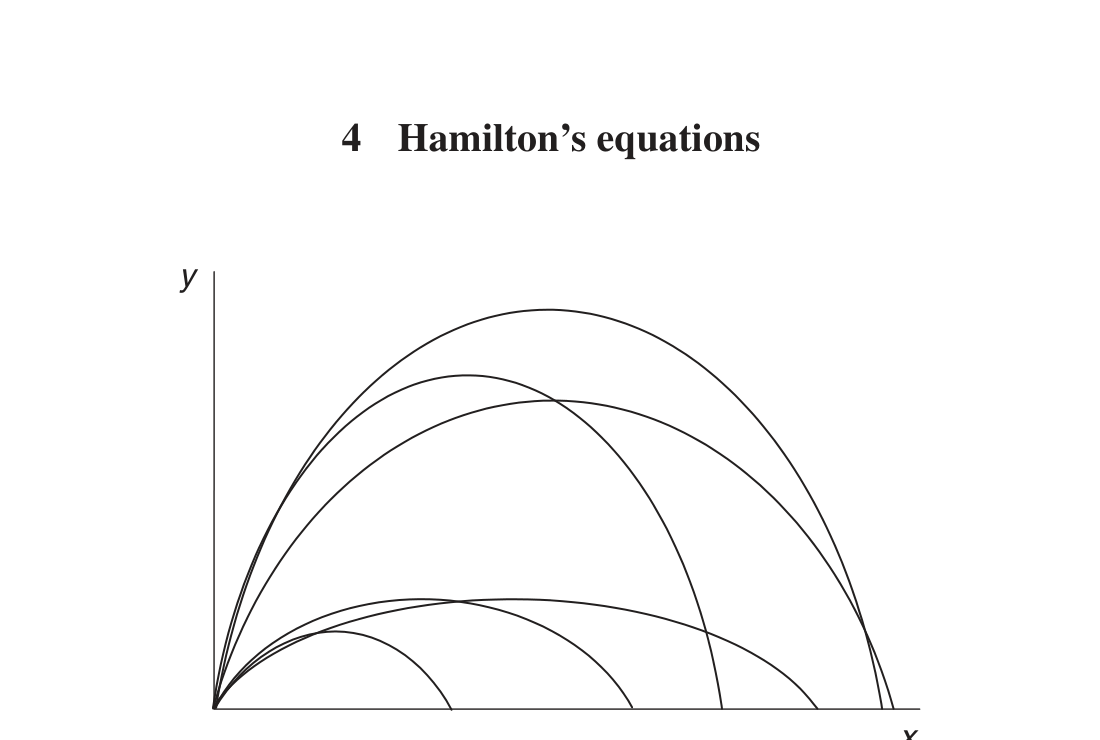
\includegraphics[width=0.55\linewidth]{../Figures/fig_4_1.png}
\caption{图 4.1}
\end{figure}

另一方面，若我们考虑从相空间中一点出发的所有可能的曲线，我们得到的将是一条唯一的曲线，因为点 $C$ 现在既包含质点的动量又包含它的位置，从而给出了初始运动方向和初始速率。从其他点出发的路径不会与从我们原来那个点出发的路径相交，因为正则方程在相空间中的每一点都确定了唯一的斜率。（当两条轨迹相交时，它们在交点处具有不同的斜率。）

从相空间中每一点出发的全部相空间曲线，可以被看作是动力学问题的通解，其中每条曲线代表某一特定初始条件下的运动。

考虑相空间曲线的另一种方式是假设系统由极多的质点组成。在某个初始时刻，每个质点都位于相空间中的一个特定点，随着时间推移，每个质点将在相空间中描绘出一条曲线。这很容易想象成与流动的河水中水分子的运动相类似。在某个初始时刻，每个水分子都有确定的位置和确定的动量。随着时间推移，水分子描绘出的流线互不相交。

这个类比非常贴切，以至于我们可以把流体力学的概念应用于相空间，并讨论“相流体”的性质。

例如，相流体在每一点的速度由正则方程 $\dot{p}_i = -\partial H/\partial q_i$ 和 $\dot{q}_i = +\partial H/\partial p_i$ 给出。这可以解释为与真实流体中的速度场相类似。流动相流体的每条流线代表系统在给定的特定初始条件下的时间演化，而相流体作为一个整体的运动则代表完整的解，即系统在任意初始条件下的时间演化。

在流体力学中，我们特别关心定常流动。若一点处的速度不随时间变化，即速度场不依赖于 $t$，我们就说该流动是定常的。若我们相流体的流动是定常的，则 $\dot{p}_i$ 和 $\dot{q}_i$ 不随时间变化，量 $\partial H/\partial q_i$ 和 $\partial H/\partial p_i$ 与时间无关，且 $H$ 不能显含时间，即 $\partial H/\partial t = 0$。但 $H$ 的全时间导数是
$$
\frac{dH}{dt} = \sum_{i=1}^{n}\left(\frac{\partial H}{\partial q_i}\dot{q}_i + \frac{\partial H}{\partial p_i}\dot{p}_i\right) = 0,
$$
其中用到了正则方程。所以
$$
\frac{dH}{dt} = 0 \implies H = \text{常数} = E .
$$
即能量守恒。此外，$H = E$ 在相空间中定义了一个曲面，质点将在该曲面上运动。我们得出结论：若能量守恒，则相流体表现得就像真实流体的定常流动一样。

我们将在下一章看到，真实流体与相流体之间还有另一个类比；即相流体将被证明表现得就像不可压缩的真实流体一样。

\section*{4.6  循环坐标与劳斯方法}

若某个坐标不出现在拉格朗日量中，则称它是循环的或可遗的。然而，拉格朗日量仍然是相应的广义速度的函数。换句话说，若 $q$ 中有一个是可遗的，则拉格朗日量只是 $n - 1$ 个广义坐标的函数，但一般而言它仍是全部 $n$ 个广义速度的函数。于是，若 $q_n$ 是可遗的，
$$
L = L(q_1, \ldots, q_{n-1}; \dot{q}_1, \ldots, \dot{q}_n; t).
$$
然而，哈密顿量将只是 $n - 1$ 个坐标和 $n - 1$ 个动量的函数，因为与可遗坐标共轭的动量是常数。例如，若 $q_n$ 是可遗的，则相应的动量 $p_n$ 是常数。让我们把它记为 $\alpha$。于是我们可以把哈密顿量写为
$$
H = H(q_1, \ldots, q_{n-1}; p_1, \ldots, p_{n-1}; \alpha; t),
\eqno\hbox{(4.21)}
$$
其中我们把常数 $\alpha$ 包含在了表达式中，尽管通常并不写出对常数的函数依赖。但事实确实如此，$H$ 确实依赖于赋予 $\alpha$ 的值。

可遗坐标 $q_n$ 不出现于哈密顿量中，但这并不意味着我们不关心它的时间演化。可遗坐标依然是处于与任何其他坐标同等地位的坐标！$q_n$ 的哈密顿方程正如你所预期的那样是
$$
\dot{q}_n = \frac{\partial H}{\partial \alpha}.
$$
常常发生的情况是，某些坐标是可遗的，而另一些不是。例如，假设一个由坐标 $q_1, \ldots, q_n$ 描述的系统，前 $s$ 个坐标出现在哈密顿量（和拉格朗日量）中，而坐标 $q_{s+1}, \ldots, q_n$ 是循环的。在这种情况下，一种处理此类问题的方法（由劳斯（Routh）提出）就派上了用场。人们定义一个称为劳斯函数（在某些方面与哈密顿量相似）的量，如下：
$$
R = \sum_{i=s+1}^{n} p_i \dot{q}_i - L.
\eqno\hbox{(4.22)}
$$
注意求和是对循环坐标进行的。于是
$$
R = R(q_1, \ldots, q_s; \dot{q}_1, \ldots, \dot{q}_s; p_{s+1}, \ldots, p_n; t).
$$
对劳斯函数关于各变量求偏导数，我们发现
$$
\frac{\partial R}{\partial q_i} = -\frac{\partial L}{\partial q_i},
\qquad i = 1, \ldots, s,
\eqno\hbox{(4.23)}
$$
$$
\frac{\partial R}{\partial \dot{q}_i} = -\frac{\partial L}{\partial \dot{q}_i},
\qquad i = 1, \ldots, s,
$$
以及
$$
\frac{\partial R}{\partial q_i} = -\dot{p}_i,
\qquad i = s + 1, \ldots, n,
\eqno\hbox{(4.24)}
$$
$$
\frac{\partial R}{\partial p_i} = \dot{q}_i,
\qquad i = s + 1, \ldots, n .
$$
方程 (4.23) 表明前 $s$ 个坐标满足以劳斯函数作为拉格朗日量的拉格朗日方程，即
$$
\frac{d}{dt}\frac{\partial R}{\partial \dot{q}_i} - \frac{\partial R}{\partial q_i} = 0,
\qquad i = 1, \ldots, s,
$$
而方程 (4.24) 表明其余的坐标和动量满足以劳斯函数作为哈密顿量的哈密顿方程。但注意，对于循环坐标 $s + 1, \ldots, n$，动量是常数，我们可以把这 $n - s$ 个动量换成常数 $\alpha_1, \ldots, \alpha_{n-s}$。于是劳斯函数可以写成
$$
R = R(q_1, \ldots, q_s; \dot{q}_1, \ldots, \dot{q}_s; \alpha_1, \ldots, \alpha_{n-s}; t).
\eqno\hbox{(4.25)}
$$
这些 $\alpha$ 可由初始条件确定，这样我们就把问题中的变量数目从 $n$ 有效减少到了 $s$。减少变量数目是求解问题的一种有力技巧。（当我们研究正则变换时，我们将遇到一种把变量数目减少到零的方法！）

劳斯函数对于分析定常运动也很方便。我们把定常运动定义为非循环变量为常数的运动。定常运动的一个例子是沿圆轨道运行的行星。在极坐标中，拉格朗日量为
$$
L = \frac{1}{2}m\dot{r}^2 + \frac{1}{2}mr^2\dot{\theta}^2 + \frac{k}{r}.
$$
对于圆轨道，非循环坐标 $r$ 是常数。坐标 $\theta$ 是循环的，并且它随时间线性增加。循环坐标的线性增加是定常运动的一个特征，这一点可以从运动方程中看出。

再举一个例子，如果我们写出一个旋转、进动的陀螺（或回转仪）的拉格朗日量，我们会发现唯一的非循环变量是极角 $\theta$。若陀螺在章动，则 $\theta$ 不再恒定，陀螺在进动的同时会“点头”。这可称为“围绕定常运动的振荡”。

就我们目前的讨论而言，非循环变量是常数。对于具有方程 (4.25) 所示形式的劳斯函数的系统，循环坐标的运动方程（方程 (4.24)）告诉我们
$$
\dot{q}_i = \dot{q}_i(q_1, \ldots, q_s; \dot{q}_1, \ldots, \dot{q}_s; \alpha_1, \ldots, \alpha_{n-s}),
\qquad i = s + 1, \ldots, n .
$$
对于定常运动，$q_1, \ldots, q_s$ 为常数，$\dot{q}_1, \ldots, \dot{q}_s$ 为零，所以 $\dot{q}_i$（$i > s$）为常数，从而 $q_i$（$i > s$）随时间线性变化。

\begin{exercise}
写出球面摆的哈密顿量。指出所有循环坐标。写出劳斯函数。
\end{exercise}

\begin{exercise}
用欧拉角写出旋转陀螺的拉格朗日量，并指出循环坐标与非循环坐标。
\end{exercise}

\section*{4.7  辛记法}

辛记法是用矩阵表示哈密顿方程的一种优雅而有力的方式。首先定义一个列矩阵 $\eta$，其元素为全部 $q$ 和全部 $p$。具体地说，对于具有 $n$ 个自由度的系统，$\eta$ 中的前 $n$ 个元素是 $q_1, \ldots, q_n$，其余 $n$ 个元素是 $p_1, \ldots, p_n$。于是 $\eta$ 有 $2n$ 个元素。接下来定义另一个 $2n$ 列矩阵，其元素是哈密顿量对全部坐标和全部动量的偏导数，因此该列矩阵的元素为
$$
\frac{\partial H}{\partial q_1}, \frac{\partial H}{\partial q_2}, \ldots, \frac{\partial H}{\partial q_n}, \frac{\partial H}{\partial p_1}, \frac{\partial H}{\partial p_2}, \ldots, \frac{\partial H}{\partial p_n}.
$$
我们把这个矩阵记为
$$
\frac{\partial H}{\partial \eta}.
$$
最后，定义一个称为 $J$ 的 $2n \times 2n$ 矩阵，其形式为
$$
J = \begin{pmatrix} 0 & -1 \\ 1 & 0 \end{pmatrix},
$$
其中 $0$ 代表 $n\times n$ 零矩阵，$1$ 代表 $n\times n$ 单位矩阵。
利用这种记法，哈密顿方程是
$$
\dot{\eta} = J\frac{\partial H}{\partial \eta}.
\eqno\hbox{(4.26)}
$$
可以注意到，这样的表达式非常适合快速的计算机计算。计算此类运动方程的计算机程序被称为“辛积分器”，广泛用于天体力学（多体问题）、分子动力学以及加速器物理中。

\begin{exercise}
证明方程 (4.26) 能够重现练习 4.6 中简谐振子的哈密顿方程。
\end{exercise}

\section*{4.8  习题}

4.1　写出双平面摆的哈密顿量。

4.2　考虑如下拉格朗日量：
$$
L = A\dot{x}^2 + B\dot{y} + C\dot{x}\dot{y} + D(x^2 + y^2) ,
$$
其中 $A$、$B$、$C$、$D$ 为常数。确定哈密顿量。

4.3　一个长为 $l$、质量为 $m$ 的平面摆以这样的方式被悬挂起来：它的悬挂点以匀速在半径为 $a$ 的竖直圆周上运动。求哈密顿运动方程。正则动量是什么？

4.4　在平面极坐标中写出绕太阳运行的行星的哈密顿量。确定哈密顿运动方程。

4.5　写出球面摆的哈密顿量及哈密顿运动方程。

4.6　用辛记法写出球面摆的哈密顿运动方程。

4.7　一个质量为 $m$ 的质点被约束在半径为 $R$ 的球面上运动（直到它从球面落下）。质点的势能为 $mgz$，其中 $z$ 从球面所放置的平面竖直向上度量。写出质点在接触球面期间的哈密顿量及哈密顿运动方程。

4.8　考虑一个正则变换。写出函数行列式，并证明 $\Delta = 1$。（函数行列式是一个行列式，其元素是一组变量对另一组变量的偏导数。每行只含一个变量的导数，每列只含对某一个变量的导数。）

4.9　一根劲度系数为 $k$ 的无质量弹簧悬挂在一个支撑点上，该支撑点以频率 $\omega$ 做竖直振动，弹簧顶端的位置为 $z_0 = A\cos\omega t$。一个质量为 $m$ 的质点系在弹簧下端。求该系统的哈密顿量。

4.10　一个质量为 $m$ 的质点可以在质量为 $M$ 的水平杆上自由滑动。杆的一端与转台相连，以角速度 $\omega$ 在半径为 $a$ 的圆周上运动。写出该系统的哈密顿量。
